\documentclass[journal,transmag,11pt]{IEEEtran}

\usepackage{graphicx}
\usepackage{stfloats}

\hyphenation{op-tical net-works semi-conduc-tor}

\begin{document}
\title{Towards Privacy Protection Composition Framework \\in Internet of Vehicles}

\author{\IEEEauthorblockN{Xiaotong Wu\IEEEauthorrefmark{1},
Xiaolong Xu\IEEEauthorrefmark{2} and
Muhammad Bilal\IEEEauthorrefmark{3}
%Montgomery Scott\IEEEauthorrefmark{3}, 
%Eldon Tyrell\IEEEauthorrefmark{4},~\IEEEmembership{Fellow,~IEEE}
}
\IEEEauthorblockA{\IEEEauthorrefmark{1}School of Computer and Electrical Information, Nanjing Normal University, PR China}
\IEEEauthorblockA{\IEEEauthorrefmark{2}School of Computer and Software, Nanjing University of Information Science \& Technology, PR China}
\IEEEauthorblockA{\IEEEauthorrefmark{3}Department of Computer and Electronic Systems Engineering, Hankuk University of Foreign Studies, Korea}

%\IEEEauthorblockA{\IEEEauthorrefmark{3}School of Information, Science and Engineering, Qufu Normal University, PR China}
\thanks{Manuscript received December 1, 2012; revised August 26, 2015. 
Corresponding author: Muhammad Bilal (Email: m.bilal@ieee.org).}}

\markboth{IEEE Consumer Electronics Manazine,~Vol.~14, No.~8, August~2015}%
{Wu \MakeLowercase{\textit{et al.}}: Towards Privacy Protection Composition Framework in Internet of Vehicles}

%\IEEEpubid{0000--0000/00\$00.00~\copyright~2015 IEEE}
%\IEEEspecialpapernotice{(Invited Paper)}

\IEEEtitleabstractindextext{%
\begin{abstract}
As an emerging computing paradigm, the Internet of Vehicles (IoV) brings a lot of benefits for drivers and consumers, such as reducing traffic congestion and parking difficulty, route recommendation, information sharing. However, participants in IoV are inevitably faced with security and privacy risks, since their data are outsourced to the third party. In this paper, we present a comprehensive analysis of the root causes of privacy risks in IoV and the corresponding solutions. At first, we introduce the concrete privacy challenges based on the structural characteristics of IoV. Then, we present a unified framework of data privacy preservation in IoV, which integrates multiple efficient private techniques, including encryption, anonymity and perturbation. Next, we investigate the possible research directions for route recommendation, charging deployment, traffic prediction under different privacy requirements in detail. We also add more emerging techniques and environments (e.g., blockchain, smart grid, 5G communication) to strengthen the ability and application of IoV.
\end{abstract}

% Note that keywords are not normally used for peerreview papers.
%\begin{IEEEkeywords}
%IEEE, IEEEtran, IEEE Transactions on Magnetics, journal, \LaTeX, magnetics, paper, template.
%\end{IEEEkeywords}
}

\maketitle

\IEEEdisplaynontitleabstractindextext

%\ifCLASSOPTIONpeerreview
% \begin{center} \bfseries EDICS Category: 3-BBND \end{center}
% \fi
\IEEEpeerreviewmaketitle

%Towards privacy preserving IoT Environments: A survey

\section{Introduction}
\IEEEPARstart{W}{ith} the fast development of communication and infrastructure technologies, the Internet of Vehicles is attracting more and more attention from academia and industry \cite{journals/tits/ChengCZLGL15}. The novel computing paradigm consists of hundreds of thousands of interacted and autonomous vehicles, which each is viewed as an intelligent object having certain ability with sensing, computing and storage resources. Intelligent entities are able to undertake multiple different roles, which brings a series of functions, including autonomous driving and platooning, information sharing and learning, traffic control and optimization.

The combination of intelligent entities and other advanced techniques greatly leads to the generation of new scenes, paradigms, applications and services. For example, vehicles are evolving from simple data consumers to intelligent agents that form the \textit{Vehicular Cloud} in a local environment to offer ample resources \cite{conf/wf-iot/GerlaLPL14}. Various techniques of artificial intelligence (e.g., deep reinforcement learning \cite{journals/tccn/NingDWGRKHK19}) are widely applied to IoV, forming a more intelligent computing paradigm, i.e., Intelligent Internet of Vehicles (IIoV). CarStream, an industrial system of big data processing, utilizes the existing big data techniques (e.g., Hadoop, Kafka) to make full use of data of vehicles to provide various services (e.g., electronic fence, vehicle tracking, order prediction) \cite{journals/pvldb/ZhangWLXL17}. Multiple-access edge computing, a special edge computing, views vehicles as a powerful computing unit, i.e., edge nodes or servers, to analyze raw data and save transmission time \cite{journals/comsur/WangLKLSXH20}.

while various advanced techniques greatly contribute to the development of Internet of Vehicles, the fundamental resource is still data of vehicles, including location information, speed, destination and so on. The efficient utilization of data addresses the grand challenges on road transportation, including traffic congestion, parking difficulties, accident rescue, pickup point deployment. Meanwhile, drivers also enjoy the corresponding benefits of sharing their data, such as accurate GPS navigation, charging and route recommendation and other personalized services and applications. 

Unfortunately, participants in IoV are inevitably faced with security and privacy risks due to the special and complex structure of IoV and strong attacks of malicious adversaries. For example, Frassinelli et al. \cite{conf/sp/FrassinelliPN20} designed a tool \textsf{AutoCAN} to reveal that car makers track the GPS position, the number of occupants, usage statistics of doors, lights, by in-vehicle networks. The findings show that sensitive information of vehicles is indeed sent to the third party, while drivers cannot know the purpose behind the collection of data. On the other hand, even if drivers are willing to share data for high-quality services, the usage of data is out of their control. It is necessary for the third party (i.e., data collectors) to adopt various measures to ensure data security. 

In recent years, there have been a series of research works from academia and industry to study data protection mechanisms in different scenes satisfying different privacy requirements. In this paper, we combine the existing works and give possible solution approaches to answer an important problem for vehicles, i.e., \textit{how to enjoy the high-quality services from the third party and get a strong security guarantee to avoid the possible privacy leakage}. 

\begin{figure*}[tbp]
	\centering
	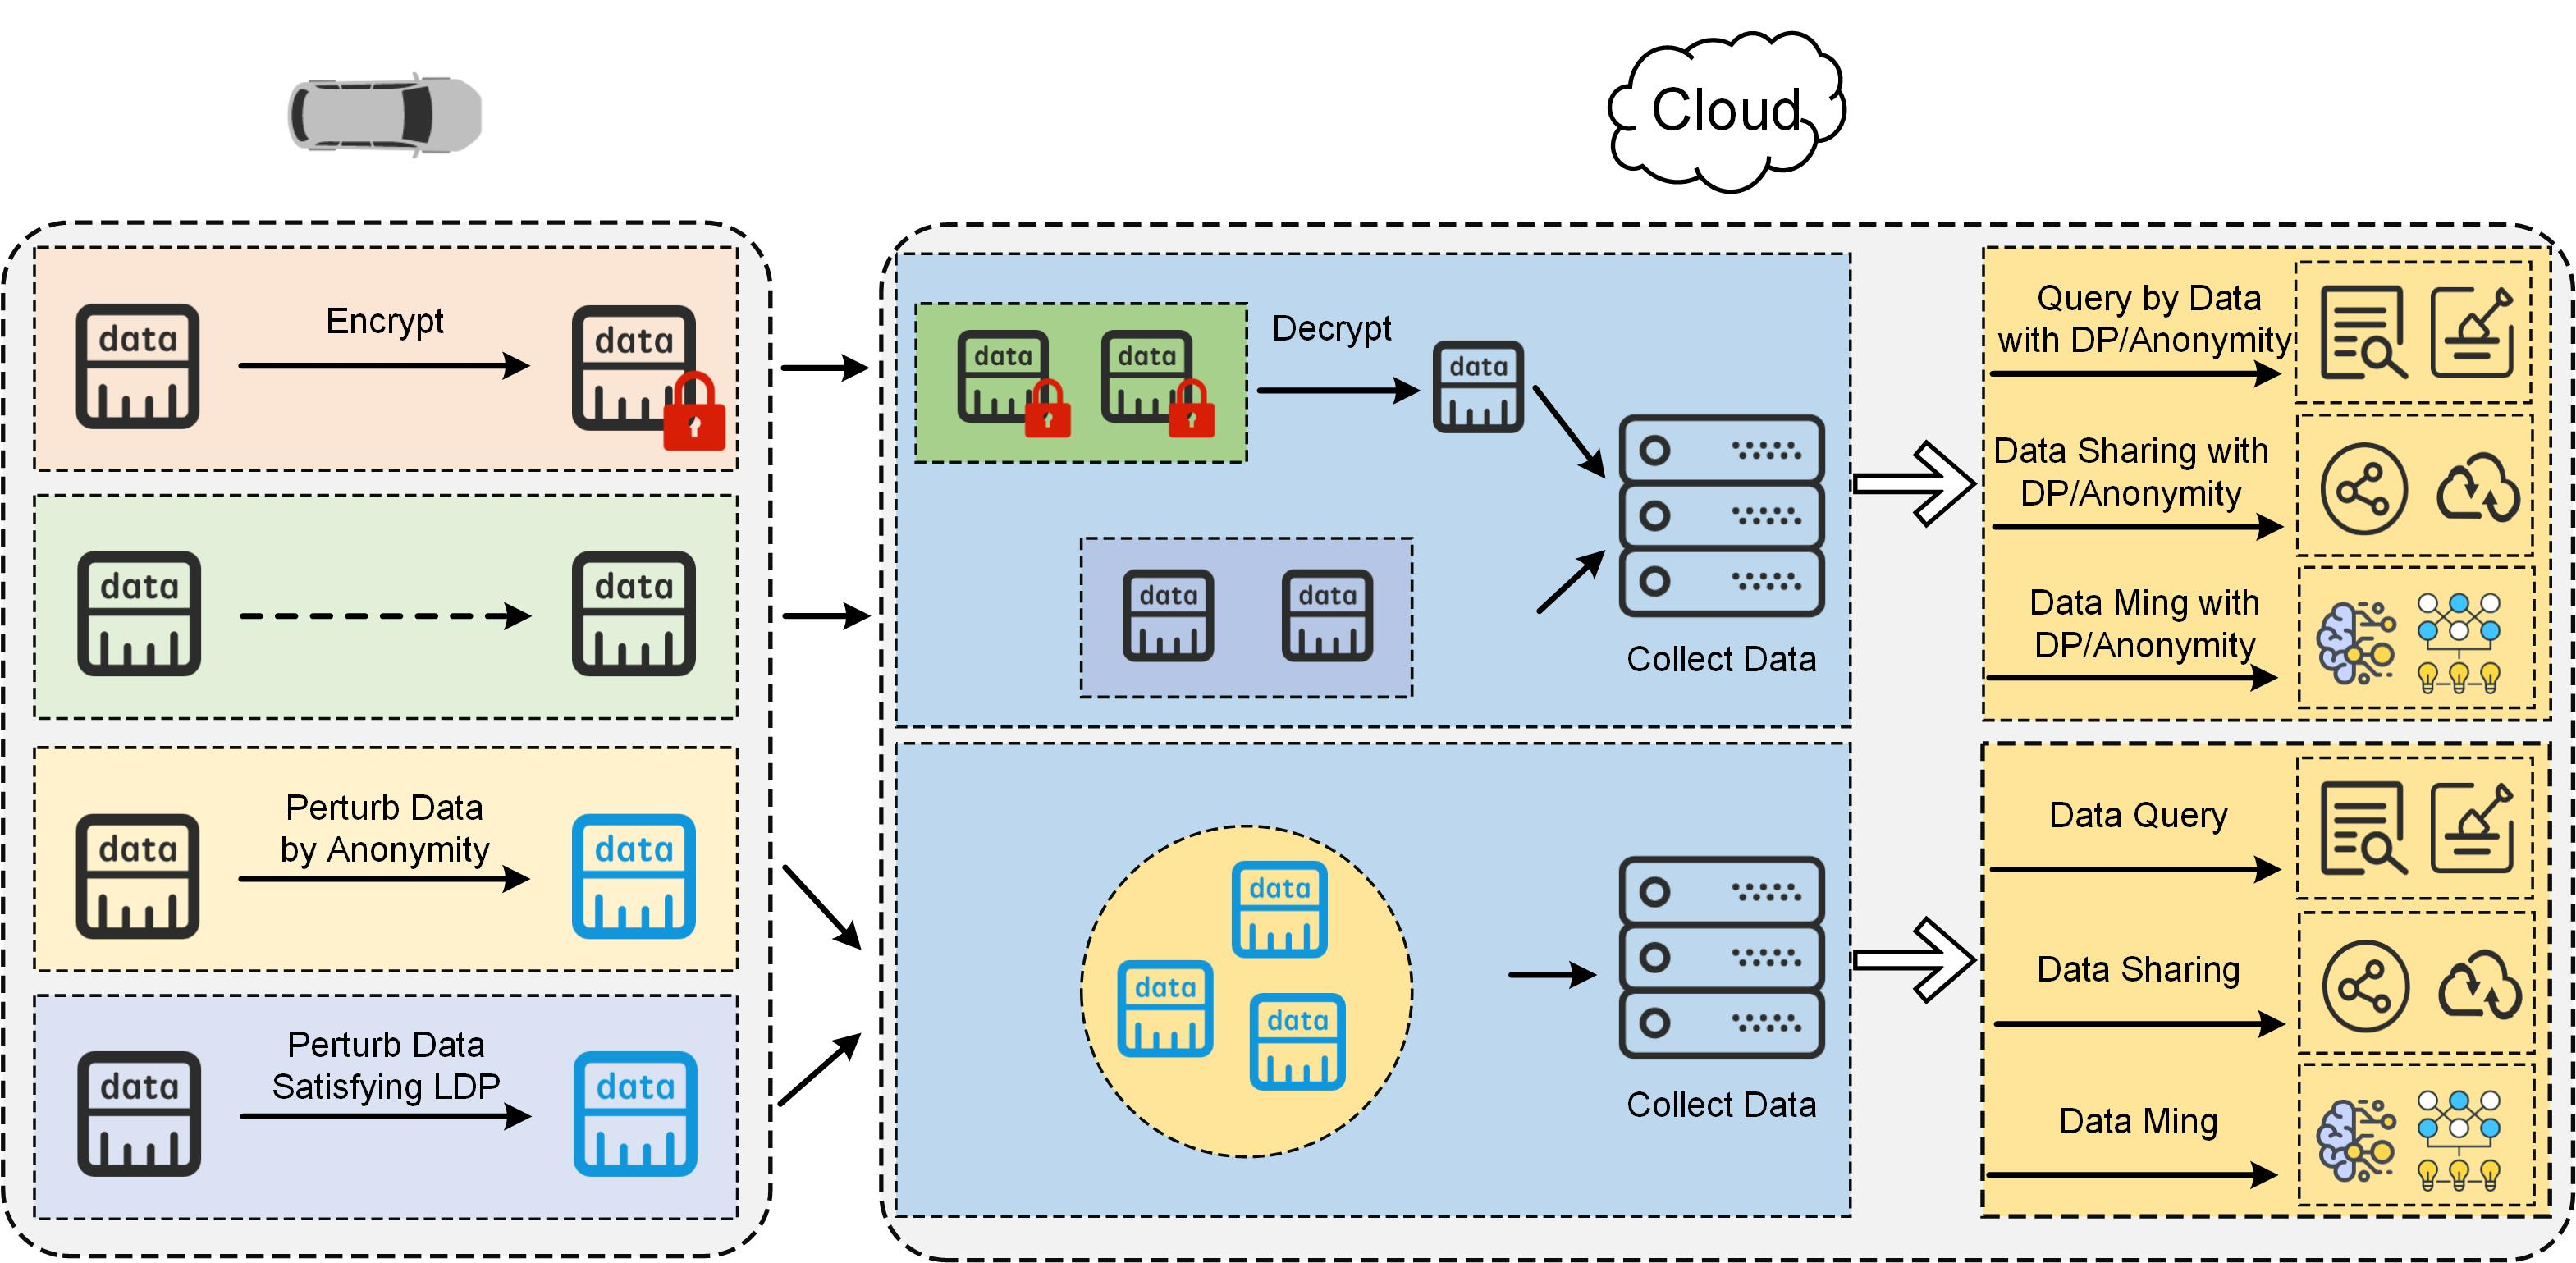
\includegraphics[width=0.98\linewidth]{framework.jpg}
	\caption{Unified Framework for Data Privacy Preservation in IoV.}
	\label{fig_framework}
\end{figure*}

\section{Privacy Challenges in IoV}
Since the intelligent Internet of Vehicles integrates the advanced techniques of multiple computing paradigms, its structure has the following characteristics:
\begin{itemize}
	\item \textbf{Complexity of Network Communication.} In IoV, there are multiple types of network communication, including vehicle-to-vehicle, vehicle-to-cloud, vehicle-to-RSU and so on. 
	\item \textbf{Limited Capability of Intelligent Vehicles.} Although intelligent vehicles have certain capability, their resources are relatively limited. It is difficult for them to process complex computing or storage tasks.  
	\item \textbf{Diversity of Intelligent Vehicles.} The capability of vehicles is not consistent. Some vehicles have the strong computational performance and others have the storage and network transmission. Meanwhile, different vehicles have different security and privacy requirements.  
\end{itemize}

The above characteristics of IoV brings the new security and privacy challenges for vehicles and the third party to protect their data: 
\begin{itemize}
	\item \textbf{Vulnerability of Network Communication.} Due to the complexity of vehicle-to-everything communications, the network is easily attacked by malicious adversaries.
	\item \textbf{Low Complexity of Protection Measures.} Protection measures with high computational complexity are difficultly applied to IoV. However, some measures with low computation cannot provide strong privacy protection.
	\item \textbf{Personalized Privacy Protection.} There are hundreds of thousands of vehicles, which each has its own protection requirement. More seriously, some malicious vehicles attempt to get the sensitive information of others.
\end{itemize}

These challenges imply that IoV needs more secure and more efficient protection mechanisms to protect a large number of vehicles with personalized privacy requirements.

\section{Framework of Privacy Preservation}

Faced with severe privacy challenges, single protection scheme is hard to provide the strong privacy guarantee to satisfy the diversity of intelligent vehicles. It is an urgent need of a framework to support diverse privacy schemes of vehicles and different performances of resources. To this end, we present a unified framework that takes full advantage of various advanced privacy protection techniques to deal with different privacy requirements under complex environments.

Fig.~\ref{fig_framework} shows a unified framework for data privacy preservation in IIoV. There are two important participants in Internet of Vehicles, i.e., the drivers and the vehicular cloud. On one hand, the drivers generally provide their raw or perturbed data to the vehicular cloud to get high-quality services. On the other hand, the outsourced data are out of the drivers' control, which makes them worried about the possible leakage. Here, according to different ways of data transmission, the operations of vehicles are classified into four cases that are listed as follows:
\begin{itemize}
	\item \textbf{Data Encryption.} The scheme is to encrypt the raw data of vehicles so as to protect the security of network communication. In advance, the vehicles and the vehicular cloud need to agree on the corresponding public and private key. Meanwhile, the vehicles undertake a certain amount of computational overhead.
	\item \textbf{Raw Data.} The scheme directly sends the raw data to the vehicular cloud. It is obvious that it has a relatively high privacy risk of network transmission. Thus, the scheme is just suited to the scene with no privacy requirement. 
	\item \textbf{Data Anonymization.} The scheme modifies the raw data and make them satisfy a certain amount of privacy requirement. However, the anonymous techniques cannot provide a strong privacy protection due to the limitation of approaches.
	\item \textbf{Data Perturbation.} Perturbation is one of the most efficient protection techniques in IoV, such as differential privacy (DP). It provides a strong privacy standard with rigorous mathematical definition. Meanwhile, the proposed privacy mechanisms need to be verified by theoretical demonstration.
\end{itemize} 	

The vehicular cloud collects raw, encrypted, perturbed data of vehicles. For different cases, there are different processing approaches. For encrypted data, it needs to be decrypted as raw data by private key. When the raw data are used for query, sharing and intelligent analysis, the vehicular cloud should adopt some privacy protection measures, which satisfy some privacy standard (e.g., anonymity, DP). Since perturbed data have been processed by some private mechanisms, it is not necessary for the vehicular cloud to adopt some measures. According to its own privacy requirement, each vehicle selects proper measures to protect its data. Meanwhile,  it is able to combine various privacy protection techniques to provide more strong protection under different scenes.

\section{Encryption-based Schemes}

Encryption is a traditional secure technique, which is used to protect data of vehicles by securing network communication. As a rising computing paradigm, IoV is also combined with other common advanced techniques to cause an increasingly important influence on the whole society.

\subsection{Blockchain}
Blockchain is a set of techniques to store data and transactions in a secure, trusted, transparent and traceable manner. As a novel decentralized distributed technology, blockchain has many remarkable and intrinsic characteristics, such as decentralization, anonymity, and auditability  \cite{journals/csur/LaoLHXGY20}. It has been widely applied to smart contracts, health care, communication systems, financial systems, communication systems. By making full use of the advantages of blockchain, the security of many distributed systems is greatly guaranteed, especially in cloud computing, Internet of Things. Thus, blockchain technology has a certain amount of potential to secure the data of vehicles and guarantee their privacy in IoV. 

It is natural to ask an important question, i.e., what scenes is blockchain suited to? Here, we give some possible solutions of blockchain to secure data of vehicles. It consists of two main aspects, including secure architecture and services with privacy guarantee. The first part is to secure vehicular communications by blockchain technology. The possible solution directions consist of (i) constructing a blockchain-based network communication to implement trusty interaction among vehicles, service and infrastructures providers, and avoid the addition of the third party, (ii) integrating vehicles to provide value-added and trusty services (e.g., resource sharing) by utilizing unalterable property of blockchain. The second part is to (i) utilize smart contracts to implement powerful authentication and authorization of accessing, sharing and exchanging data among connected vehicles, (ii) provide privacy-shielding services for charging electric vehicles by bitcoin, and (iii) offer blockchain-based searching and matching of electric vehicles charging demander that considers the reputation of suppliers.

\subsection{Smart Grid}
The smart grid is a modernized electrical power system to have the advanced functions of power monitoring and management, which consists of intelligent charging points \cite{journals/tits/RigasRB15}. For some drivers, they need to pay to charge for electric vehicles. Therefore, there are two important privacy challenges, including vehicle-to-grid communication and data collection by charging points. On one hand, the malicious adversaries possibly launch the attack to get information of network communication. On the other hand, drivers' sensitive information (e.g., location, payment) is collected by the third party. However, it is possible for the third party to utilize side information to get sensitive information of drivers. Thus, for two cases, it is necessary to adopt efficient measures to protect communication security and data privacy.

Here, we give several possible solutions to guarantee the security and privacy of IoV. They are (i) designing an privacy-preserving authentication scheme by the traditional encryption techniques to implement efficient and secure key establishment and agreement, (ii) providing an encryption-based payment mechanism to preserve the payment information from possible leakage. For data privacy of vehicles, the encryption-based techniques can not provide security and privacy guarantee, when the third party is untrusted.

\subsection{5G Communication}
5G is an emerging communication technique, which greatly increases the speed of network transmission \cite{journals/pieee/LuZNF20}. As the application of 5G, it provides vehicle-to-everything in IoV to support networking connections among vehicles, sensors, charging points, RSUs. On the other hand, it contributes to the development of driverless cars, since the communication delay is greatly reduced. However, it also brings a series of trust, security, privacy issues toward vehicles. In special, there are a lot of malicious attacks, such as packet analysis/tracing attacks, linkage attacks, identity revealing attacks, inference attacks, deanonymization/reidentification attacks.

5G brings both opportunities and challenges for data privacy preservation in IoV. On one hand, it greatly decreases the delay of communication among vehicles and other devices, since it offers high rates anytime and anywhere. On the other hand, the high mobility of vehicles with 5G causes the uncertainty of scenes. That is, for each vehicle, its neighbor vehicles and sensors change, all the time. It is an urgent need of encryption-based privacy schemes to implement secure protection. Here, the main focus is on the computational overhead of vehicles, due to their limited capability.

\section{Anonymity-based Schemes}

Encryption-based mechanisms usually do not change the raw data of vehicles and thus have no influence on data utility. However, they only protect the communication security of vehicles. When the third party is not trusted, it can not offer the strong privacy protection. Instead, anonymity-based scheme modify the raw data to address the problem, which also causes a certain amount of data loss.

\subsection{Location-based Services}

Location information is one of the most-widely used data in IoV. There are a lot of services based on location of vehicles, including GPS navigation, traffic prediction. Meanwhile, location is also one of the most sensitive data of drivers. Most of them are unwilling that their location is leaked to others.

There are a lot of anonymous schemes to protect location information, such as $k$-anonymity \cite{conf/icc/WuLYD17}, mix-zone \cite{journals/tvt/YingMH15}, pseudonyms \cite{journals/comsur/ContiWC13}. $k$-anonymity is to merge $k$ trajectories to one, which makes adversaries not distinguish them. Mix-zone is a specified area, in which all the vehicles adopt some protection measures to satisfy some privacy requirement together. In most scenes, drivers use pseudonyms to replace their real identifies. However, the long term use of a pseudonym has little protection effect. Therefore, it is necessary to design proper measures to incentive drivers to update their pseudonyms. Here, the combination of multiple anonymous techniques increases the privacy protection level of vehicles. Since the techniques cause utility loss, it is worthwhile considering the balance between privacy strength and data utility. Relatively speaking, the anonymous techniques can not give the theoretical analysis to rigorously demonstrate the privacy protection effect.  

\subsection{Anonymous Charging and Billing}

Charging and billing are one of the most common operations for charging of electric vehicle and fuel charging of normal cars in IoV. Charing for vehicles may cause the location leakage of drivers, since the sensitive information is outsourced to the third party. Billing for payment also consists of a large amount of sensitive information, such as location, time, cost. How to protect the data is an extremely challenging problem.

Anonymous techniques are one of the most efficient and simplest approaches for vehicles. Different from location-based services, charging and billing consists of more formats of data. The basic operation of vehicles is to replace the real identity with pseudonyms. After it collects the data from vehicles, the vehicular cloud utilizes some typical anonymous techniques to process multidimensional data, such as $k$-anonymity \cite{conf/icc/WuLYD17}, $l$-diversity \cite{conf/icde/MachanavajjhalaGKV06}, $t$-closeness \cite{conf/icde/LiLV07}. As a result, the vehicular cloud is able to offer data sharing, data-based query, data mining-based services. On the other hand, it is an interesting topic to research the incentive measures to motive vehicles to offer more accurate data.


\section{Differential Privacy}

Similar to anonymity-based schemes, some mechanisms satisfying differential privacy perturb the raw data of vehicles, which also cause a certain amount of utility loss. However, differential privacy is a stronger privacy standard, which is a rigorous mathematical model \cite{conf/tamc/Dwork08}. It assumes that the third party (e.g., the vehicular cloud) is trusted and executes the perturbation operations. Here, we consider two important scenes to analyze the privacy protection, i.e., data query and artificial intelligence.

\subsection{Data Query}

Data query is a basic data sharing service provided by the vehicular cloud. If it directly answers the query questions based on the raw data, the information of vehicles is possibly leaked. For example, there are two simple queries, (i) How many drivers are in New York? and (ii) Except of Jack, how many drivers are in New York? By the queries, the adversary knows whether or not Jack is in New York. The simple example shows that the adversaries use the combination of queries to get sensitive information of vehicles.

It is necessary to adopt some measures to increase the privacy of vehicles. Fortunately, there are some effective mechanisms satisfying differential privacy to achieve the purpose. For example, Laplace mechanism adds a certain amount of noise to the real answer, while the exponential mechanism outputs some answer derived from some probability \cite{conf/tamc/Dwork08}. However, these simple mechanisms can not be directly applied to IoV, since there are more complex data and environments. It should design a novel privacy framework with efficient mechanisms to satisfy the special environment. It also considers the utility, since the raw data are perturbed.  

\subsection{Artificial Intelligence}

As an intelligent object, each vehicle is equipped with various sensors and devices and thus has a capability of computation, storage, communications. It is an important challenge to take advantage of intelligent entities to provide good services by deep learning, machine learning, federating learning. Meanwhile, it is also faced with privacy risk for the novel intelligent model.

There are two classes of privacy problems in the combination of artificial intelligence and IoV. The first one is that the parameters of training models are possibly leaked to the adversary by various attacks. The second one is that the data of vehicles used for training is leaked to the adversary. The privacy problems greatly hinder the application of artificial intelligence to IoV. In order to solve the above problems, it is necessary to adopt proper measures to ensure the privacy. Compared to other privacy metrics, differential privacy has stronger and more rigorous standard. The possible research directions are utilizing deep learning, machine learning to provide high-quality services (e.g., route scheduling), which also satisfy differential privacy.

\section{Local Differential Privacy}

Local differential privacy is an extended version of differential privacy, which is suited to the local setting \cite{conf/focs/DuchiJW13}. It assumes that the data collector is not trusted and requires that vehicles should adopt some randomized mechanisms to protect their own data. Compared to differential privacy, it defines a more rigorous privacy and avoids all possible leakage risks, except of drivers. It is well suited for vehicles to ensure their own privacy and undertake the cost of quality of services.

\subsection{Edge/Fog Computing}

Edge/Fog computing is a distributed computing paradigm, in which data analysis is executed in the network edge to reduce the communication delay. It is a potential structure, which is well suited to IoV and makes full use of resources of vehicles. Meanwhile, local differential privacy is to strengthen the protection level of vehicles. 

At present, the researchers from academia and industry just study the basic mechanisms satisfying local differential privacy, including frequency estimation, heavy hitter identification, itemset mining, marginal release. Relatively speaking, there are few works to study data mining, key-value data collection, private spatial data aggregation. Therefore, there are yet open problems to design privacy protection mechanisms satisfying local differential privacy in various aspects of IoV.

%\begin{figure*}[!t]
%\centering
%\subfloat[Case I]{\includegraphics[width=2.5in]{box}%
%\label{fig_first_case}}
%\hfil
%\subfloat[Case II]{\includegraphics[width=2.5in]{box}%
%\label{fig_second_case}}
%\caption{Simulation results for the network.}
%\label{fig_sim}
%\end{figure*}

%\begin{table}[!t]
%% increase table row spacing, adjust to taste
%\renewcommand{\arraystretch}{1.3}
% if using array.sty, it might be a good idea to tweak the value of
% \extrarowheight as needed to properly center the text within the cells
%\caption{An Example of a Table}
%\label{table_example}
%\centering
%% Some packages, such as MDW tools, offer better commands for making tables
%% than the plain LaTeX2e tabular which is used here.
%\begin{tabular}{|c||c|}
%\hline
%One & Two\\
%\hline
%Three & Four\\
%\hline
%\end{tabular}
%\end{table}

\section{Conclusion}

The main focus of the paper is on the privacy protection problems in IoV. We first presented the possible privacy challenges in IoV due to its structural characteristics. We gave a unified framework for data privacy preservation to make full use of the existing private techniques. Combined with various advanced techniques, we presented the possible research directions of IoV.

% if have a single appendix:
%\appendix[Proof of the Zonklar Equations]
% or
%\appendix  % for no appendix heading
% do not use \section anymore after \appendix, only \section*
% is possibly needed

% use appendices with more than one appendix
% then use \section to start each appendix
% you must declare a \section before using any
% \subsection or using \label (\appendices by itself
% starts a section numbered zero.)
%


%\appendices
%\section{Proof of the First Zonklar Equation}
%Appendix one text goes here.

% use section* for acknowledgment
\section*{Acknowledgment}

This work was supported in part by the National Natural Science Foundation of China under Grant No. 41971343, No. 61872422, No. 41771411.

% Can use something like this to put references on a page
% by themselves when using endfloat and the captionsoff option.
\ifCLASSOPTIONcaptionsoff
  \newpage
\fi



% trigger a \newpage just before the given reference
% number - used to balance the columns on the last page
% adjust value as needed - may need to be readjusted if
% the document is modified later
%\IEEEtriggeratref{8}
% The "triggered" command can be changed if desired:
%\IEEEtriggercmd{\enlargethispage{-5in}}

% references section

% can use a bibliography generated by BibTeX as a .bbl file
% BibTeX documentation can be easily obtained at:
% http://mirror.ctan.org/biblio/bibtex/contrib/doc/
% The IEEEtran BibTeX style support page is at:
% http://www.michaelshell.org/tex/ieeetran/bibtex/
\bibliographystyle{IEEEtran}
% argument is your BibTeX string definitions and bibliography database(s)
\bibliography{refs}
%
% <OR> manually copy in the resultant .bbl file
% set second argument of \begin to the number of references
% (used to reserve space for the reference number labels box)
%\begin{thebibliography}{1}

%\bibitem{IEEEhowto:kopka}
%H.~Kopka and P.~W. Daly, \emph{A Guide to \LaTeX}, 3rd~ed.\hskip 1em plus
%  0.5em minus 0.4em\relax Harlow, England: Addison-Wesley, 1999.

%\end{thebibliography}

% biography section
% 
% If you have an EPS/PDF photo (graphicx package needed) extra braces are
% needed around the contents of the optional argument to biography to prevent
% the LaTeX parser from getting confused when it sees the complicated
% \includegraphics command within an optional argument. (You could create
% your own custom macro containing the \includegraphics command to make things
% simpler here.)
%\begin{IEEEbiography}[{\includegraphics[width=1in,height=1.25in,clip,keepaspectratio]{mshell}}]{Michael Shell}
% or if you just want to reserve a space for a photo:

%\begin{IEEEbiography}{Michael Shell}
%Biography text here.
%\end{IEEEbiography}

% if you will not have a photo at all:
\begin{IEEEbiographynophoto}{Xiaotong Wu}
	received his Master and PhD degree at the Department of Computer Science and Technology, Nanjing University, China. He has received the B.S. degree in Software Engineering from Central South University. Now, he is an assistant professor in School of Computer and Electronic Information, Nanjing Normal University, China. His research interests include artificial intelligence, data privacy, network security, cloud computing and big data.
\end{IEEEbiographynophoto}

% insert where needed to balance the two columns on the last page with
% biographies
%\newpage

\begin{IEEEbiographynophoto}{Xiaolong Xu}
	received the Ph.D. degree in computer science and technology from Nanjing University, Nanjing, China, in 2016. He was a Research Scholar with Michigan State University, East Lansing, MI, USA, from 2017 to 2018. He is currently a Professor with the School of Computer and Software, Nanjing University of Information Science and Technology, Nanjing, China. He has authored or coauthored more than 100 peer-review articles in international journals and conferences, including IEEE TITS, IEEE TII, ACM TOIT, ACM TOMM, IEEE IOT, IEEE TCC, IEEE TBD, IEEE TCSS, IEEE TETCI, IEEE ICWS, ICSOC, etc. Among them, 10 papers are selected as the ESI Highly Cited Papers and 8 of them are selected as the ESI Hot Paper. His research interests include edge computing, the Internet of Things (IoT), cloud computing, and big data. Prof. Xu is a fellow of EAI (European Alliance for Innovation). He was the recipient of the Best Paper Award from the CBD 2016, IEEE CPSCom 2020, and SPDE 2020, the distinguish paper award from EAI Cloudcomp 2019, the best student paper award from EAI Cloudcomp 2019, and the Best Session Paper Award from IEEE DSAA 2020.  
\end{IEEEbiographynophoto}


\begin{IEEEbiographynophoto}{Muhammad Bilal}
	received the B.Sc. degree in computer systems engineering from the University of Engineering and Technology Peshawar, Pakistan, in 2008, the M.S. degree in computer engineering from Chosun University, Gwangju, South Korea, in 2012, and the Ph.D. degree in information and communication network engineering from the School of Electronics and Telecommunications Research Institute (ETRI), Korea University of Science and Technology, in 2017. From 2017 to 2018, he was with Korea University, where he was a Postdoctoral Research Fellow with the Smart Quantum Communication Center. Since 2018, he has been an Assistant Professor with the Division of Computer and Electronic Systems Engineering, Hankuk University of Foreign Studies, Yongin, South Korea. His research interests include design and analysis of network protocols, network architecture, network security, the IoT, named data networking, blockchain, cryptology, and future internet. 
	He serves as an Editor for the IEEE Future Directions Ethics and Policy in Technology Newsletter and the IEEE Internet Policy Newsletter.
\end{IEEEbiographynophoto}



% You can push biographies down or up by placing
% a \vfill before or after them. The appropriate
% use of \vfill depends on what kind of text is
% on the last page and whether or not the columns
% are being equalized.

%\vfill

% Can be used to pull up biographies so that the bottom of the last one
% is flush with the other column.
%\enlargethispage{-5in}



% that's all folks
\end{document}


